\documentclass[a4paper,11pt,final]{article}
\usepackage{fancyvrb, color, graphbox, hyperref, amsmath, url}
%\usepackage{palatino}
\usepackage{pygments}
\usepackage[a4paper,text={16.5cm,25.2cm},centering]{geometry}
\usepackage{lipsum}
\usepackage[labelformat=simple,position=top]{subcaption}
% \renewcommand\thesubfigure{\alph{subfigure})}
\hypersetup{
  pdfauthor = {Srdjan Sarikas},
  pdftitle={Intracellular Receptors},
  colorlinks=TRUE,
  linkcolor=black,
  citecolor=red,
  urlcolor=navy
}

%\setlength{\parindent}{0pt}
%\setlength{\parskip}{1.2ex}

\title{Intracellular Receptors \\ {\small Materials and Methods: Analysis and Processing}}

\author{Srdjan}
\date{\today}

\begin{document}
\maketitle

%<<echo=False>>=
%import matplotlib.pyplot as plt
%import numpy as np
%import pandas as pd
%from islets import load_regions
%@

A typical experiment involving imaging of pancreatic slices in our lab concerns a single field of view (FOV)
showing 10s-100s of cells, in a recording of at least several, often dozens, of gigabytes.
Current tools (ImageJ, \dots) rely on loading the recording, or its part, into memory, for viewing, analysis, and processing.
It also requires laborious and long human engagement.
We have developed a set of interdependent tools to automatize as much as possible the pipeline. 
The crucial elements of our pipeline are the following:
\begin{itemize}
\item (Semi-)automatic detection of regions of interest (ROIs);
\item Transformation of ROI time traces into standard score ("z-score");
\item Quantification of the phenotype for each ROI in terms of the distribution of events of different durations.
\end{itemize}

Our toolset is inspired and relies on CaImAn \cite{giovannucci2019caiman}, a similar package developed for the purposes in neuroscience reseach.

\begin{figure}[h]
\centering
\includegraphics[width=17cm,trim=1.5cm 1.5cm 1cm 1.5cm,clip]{figures/pipeline.pdf}
\label{fig:pipeline}
\caption{
An illustration of our processing and analysis pipeline:
({\it i})  From a full movie ($T{\times}x{\times}y$), we calculate the mean (or other statistic) across all frames.
({\it ii}) We pass the mean image through a band-pass filter and define ROIs by detecting local peaks.
({\it iii}) We save ROIs with all the important information (time traces, ROI coordinates, movie statistics, recording frequency, pixel size, etc.).
({\it iv}) Traces contain features at very different time scales---with different timescales presumably important for different cell types. We collect them into separable events for analysis.
}
\end{figure}

\section{(Semi-)Automatic Detection of Regions of Interest}

When the recording is stable, obtainaing a mean image, or any other statistic over frame, is rather trivial. In case there is horizontal movement, it can be corrected for by aligning the frames to a template. For this we use the functionality present in CaImAn, except that high frequency recordings need to be rebinned to some moderate frequency (a few Hz), before correcting, in order to reduce the noise level. Once the translation offsets are obtained, we use them to correct the recording in original frequency.

To define regions of interest, we blurr the representative image by a kernel of the size we expect cells to be, 
and at the scale double of that.
The difference between these two images represents a band-pass filter of the original, where the local intensity variation are very prominent (see fig.\ref{fig:regions}B).
We then pass through all pixels where the value of the filtered image is positive (or larger than a small positive threshold), and for each pixel we search for a local peak in its vicinity. 
All the pixels that lead to the same local peak are then grouped into a single ROI.



\begin{figure}[t]
\centering
\begin{tabular}{ll}
{\fontfamily{phv}\selectfont A} & 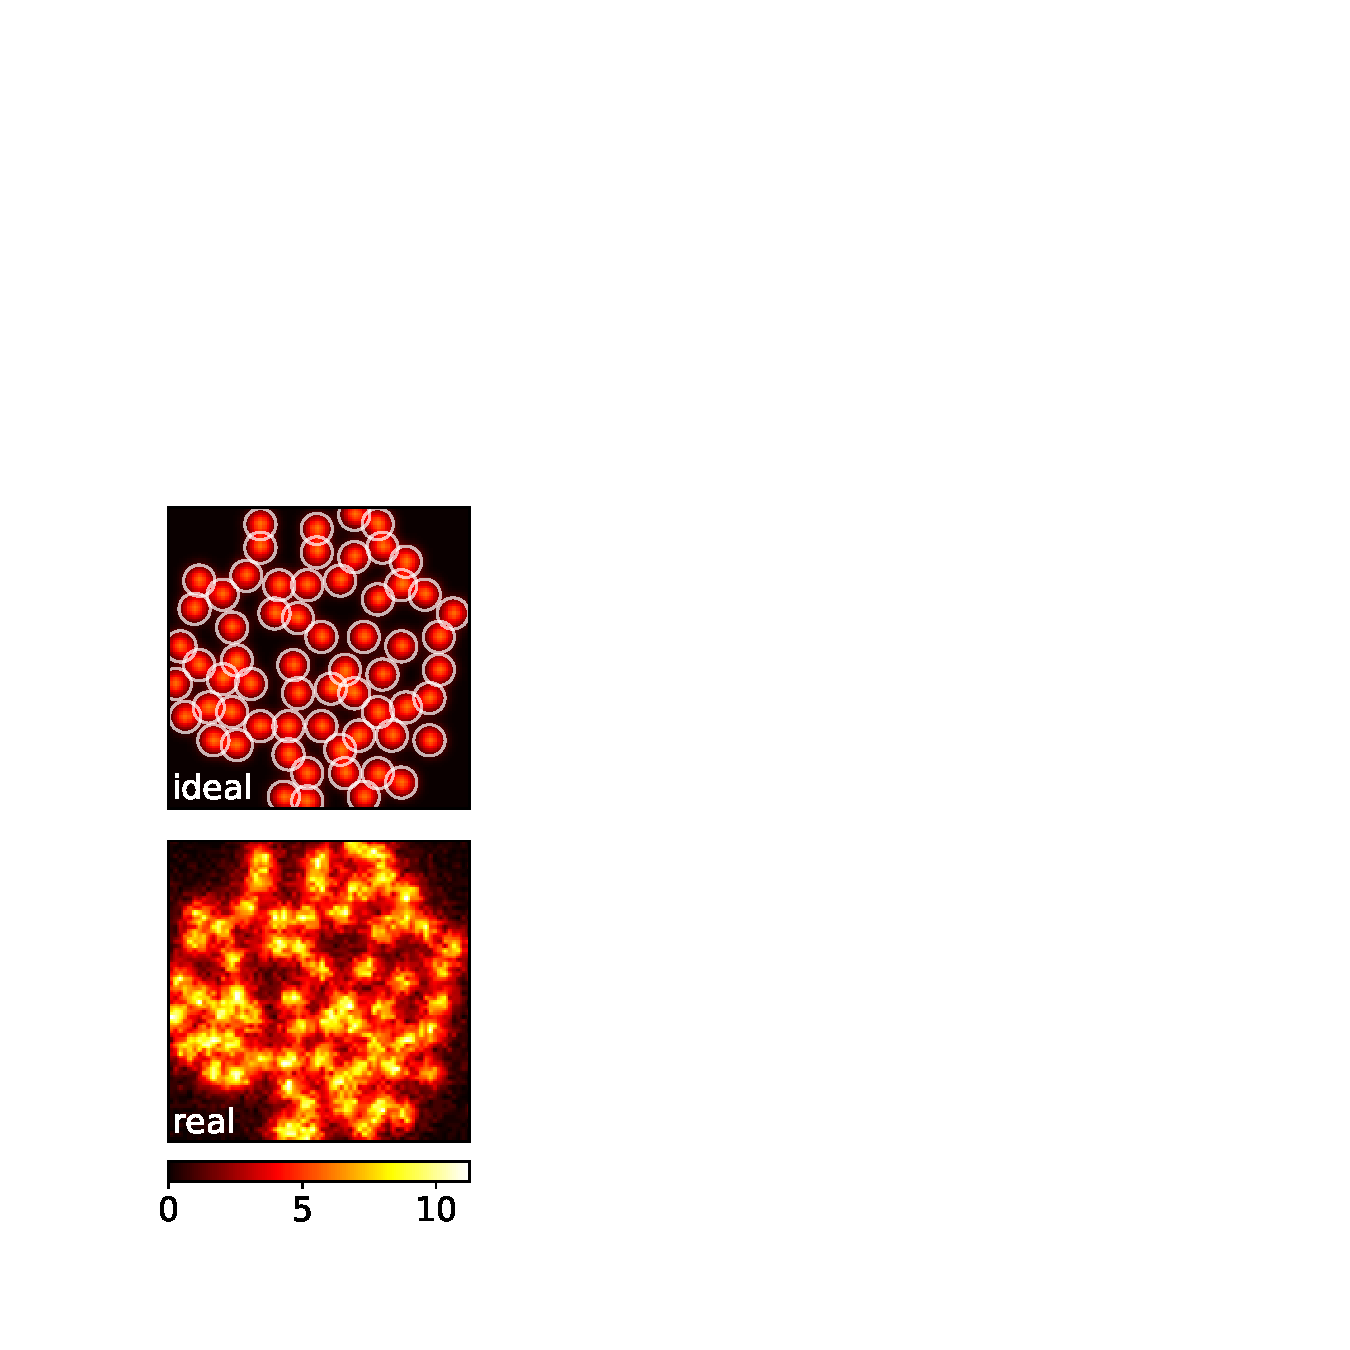
\includegraphics[scale=0.5,align=t]{figures/regions_ideal_real.pdf}\\
{\fontfamily{phv}\selectfont B} & \hspace{-5mm}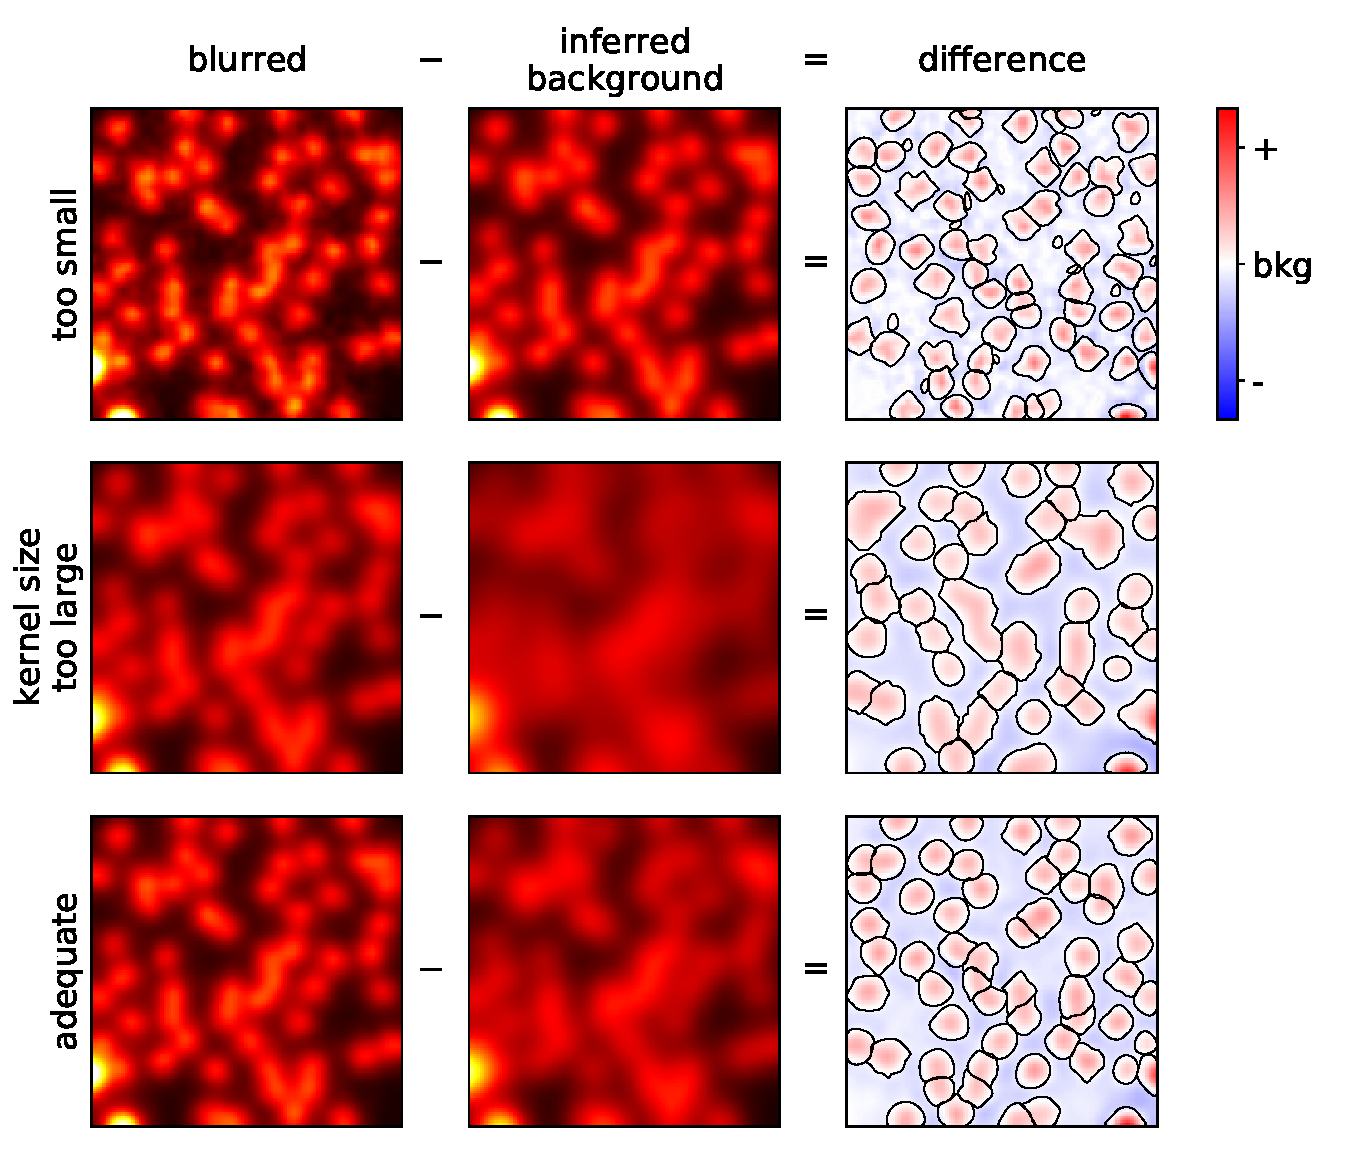
\includegraphics[scale=0.55,align=t]{figures/regions_kernels.pdf}
\end{tabular}
\caption{(A) Computationally created template image with and without noise. (B) Band-pass filtering of the "realistic" image from A, with different kernel sizes. The size of the kernel determines the approximate size of the ROIs obtained. The real locations of the cells are shown in green.\label{fig:regions}}
\end{figure}

\bibliographystyle{plain}
\bibliography{matmet}


\end{document}
